\subsection{SPI driver}

We've tried implementing a general SPI driver using C++ templates, where valid Data order, Mode and Prescale options can be specified at compile time. Thereby constructing a very specific SPI interface for the system. 

This section will focus on how to enable the SPI driver to communicate with the PCD8544.

\subsubsection{Setup}

To setup the SPI hardware on the ATmega32, we, mainly, have to modify the SPCR register\cite[136]{atmel:mega32}. The register can be seen in Figure~\ref{fig:spcr}.

\begin{figure}
	\centering
	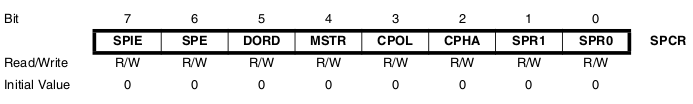
\includegraphics[width=.9\textwidth]{implementation/mega32_spcr}
	\caption{The SPCR register on the ATmega32\cite[136]{atmel:mega32}}
	\label{fig:spcr}
\end{figure}

Given the register in Figure~\ref{fig:spcr}, we enable SPI by setting SPE to one. We are also interested in establishing, the relationship of our two devices, such that the ATmega32 is master, and the PCD8544 is slave. This is done by setting MSTR to one\cite[137]{atmel:mega32}.

\subsubsection{Data order}

According to the PCD8544 data sheet, the MSB of a byte is transmitted first\cite[11]{philips:pcd8544}. Given this information, we have to set DORD to zero\cite[136]{atmel:mega32}.

\subsubsection{Mode}

By Mode, we refer to the clock polarity and the clock phase. According to the PCD8544 data sheet, the clock polarity has to be leading edge rising and trailing edge falling\cite[12]{philips:pcd8544}. Thus, CPOL in Figure~\ref{fig:spcr} has to be set to zero\cite[137]{atmel:mega32}. The data connection is sampled at rising edge\cite[11]{philips:pcd8544}, so CPHA has to be set to zero, because of leading edge sample\cite[137]{atmel:mega32}.

\subsubsection{Prescale}

We have chosen to prescale with $f_{\text{osc}}/4$, because the max clock frequency of the PCD8544 is 4MHz, as seen in Figure~\ref{fig:pcd8544_ac}. We chose this because the max frequency of the ATmega32 is 16MHz. So given an external XTAL that provides 16MHz, then our display should still function. 

\begin{figure}
	\centering
	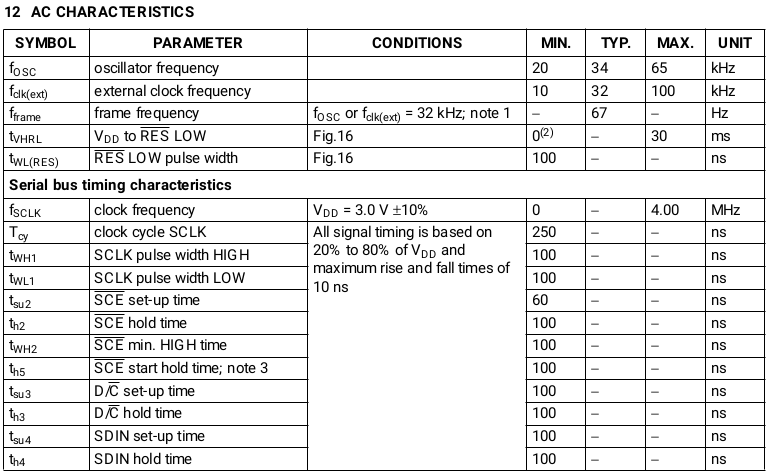
\includegraphics[width=.9\textwidth, trim={0mm 80mm 0mm 60mm}, clip]{implementation/pcd8544_ac}
	\caption{Clock frequency for the PCD8544\cite[20]{philips:pcd8544}}
	\label{fig:pcd8544_ac}
\end{figure}

